\section{Introduction}

Load following has given natural gas an economic edge over nuclear power
because natural gas plants can follow grid demand and even shut off when
renewable penetration makes the
price of electricity go negative \cite{keppler_carbon_2011}. Some French nuclear
plants have been retrofitted for load following capabilities to follow daily
variations in electricity demand \cite{lokhov_technical_2011}. Unlike the United
States, French nuclear power plants enjoy a majority share of the country's
electric generation which makes daily variations predictable. Renewable energy
has challenged the base load electricity production that
nuclear provides in the United States by introducing grid demand variability
that is much less predictable. This lack of predictability is primarily due to
renewables' tight coupling with chaotic weather systems. Figure \ref{fig:vre}
shows
that daily variations in electricity demand are reasonably predictable, with a
usual evening minimum at 40 MW. When renewable energy is included in the mix,
demand is much harder to follow.

\begin{figure}[h]
  \centering
  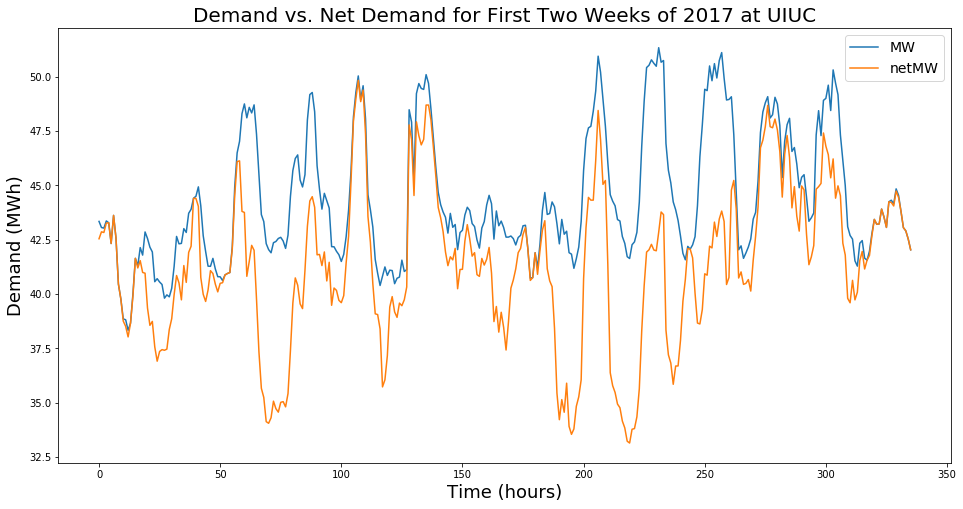
\includegraphics[width=\columnwidth]{renewable_variability}
  \caption{Comparison between total demand and demand accounting for renewable
   energy. ``NetMW'' is the wind and solar production subtracted from the
   total.}
  \label{fig:vre}
\end{figure}

Advanced reactor designs, like \glspl{MSR}, promise strong load following
capabilities due to harder
neutron spectra and faster Xe-135 burnup \cite{rykhlevskii_impact_2019}.

Unfortunately, the most mature MSR
designs are at least a decade away from obtaining a commercial license in the
United States. The climate crisis is too urgent to wait this long for nuclear
power to become fully competitive with natural gas.
Nuclear energy can be more economically feasible by relaxing the strong load
following requirements
with high fidelity predictions of renewable energy production several hours or
days in advance. If reactor operators knew in advance how much electricity will
be produced by renewable energy they
can slowly and accurately ramp reactor power to meet demand rather than operate
continuously at full power and risk paying to export electricity. Thus, relaxed
load following
improves nuclear energy's comptetitiveness against natural gas and
strengthens nuclear's ability to couple with renewable energy.
In this work we introduce \acrfull{ESN} as a preferred method for time
series forecasting of chaotic systems like electricity
production from renewable sources.
